% !TeX encoding = UTF-8
% !TeX spellcheck = pl_PL

% $Id:$

%Author: Wojciech Domski
%Szablon do ząłożeń projektowych, raportu i dokumentacji z steorwników robotów
%Wersja v.1.0.0
%


%% Konfiguracja:
\newcommand{\kurs}{Sterowniki robot\'{o}w}
\newcommand{\formakursu}{Projekt}

%odkomentuj właściwy typ projektu, a pozostałe zostaw zakomentowane
\newcommand{\doctype}{Za\l{}o\.{z}enia projektowe} %etap I
%\newcommand{\doctype}{Raport} %etap II
%\newcommand{\doctype}{Dokumentacja} %etap III

%wpisz nazwę projektu
\newcommand{\projectname}{Theremin}

%wpisz akronim projektu
\newcommand{\acronim}{THR}

%wpisz Imię i nazwisko oraz numer albumu
\newcommand{\osobaA}{Cyprian \textsc{Hryniuk}, 235512}
%w przypadku projektu jednoosobowego usuń zawartość nowej komendy
\newcommand{\osobaB}{Tomasz \textsc{Mas\l{}o\'n}, 235827}

%wpisz termin w formie, jak poniżej dzień, parzystość, godzina
\newcommand{\termin}{srTN17}

%wpisz imię i nazwisko prowadzącego
\newcommand{\prowadzacy}{mgr in\.{z}. Wojciech \textsc{Domski}}

\documentclass[10pt, a4paper]{article}

\include{preambula}
\graphicspath{{./img/}}

\begin{document}

\def\tablename{Tabela}	%zmienienie nazwy tabel z Tablica na Tabela

\begin{titlepage}
	\begin{center}
		\textsc{\LARGE \formakursu}\\[1cm]		
		\textsc{\Large \kurs}\\[0.5cm]		
		\rule{\textwidth}{0.08cm}\\[0.4cm]
		{\huge \bfseries \doctype}\\[1cm]
		{\huge \bfseries \projectname}\\[0.5cm]
		{\huge \bfseries \acronim}\\[0.4cm]
		\rule{\textwidth}{0.08cm}\\[1cm]
		
		\begin{flushright} \large
		\emph{Skład grupy:}\\
		\osobaA\\
		\osobaB\\[0.4cm]
		
		\emph{Termin: }\termin\\[0.4cm]

		\emph{Prowadzący:} \\
		\prowadzacy \\
		
		\end{flushright}
		
		\vfill
		
		{\large \today}
	\end{center}	
\end{titlepage}

\newpage
\tableofcontents
\newpage

%Obecne we wszystkich dokumentach
\section{Opis projektu}
\label{sec:OpisProjektu}

Celem projektu jest stworzenie theremina opartego na płytce rozwojowej STM32L476G-DISCO\cite{DevBoard} i dwóch cyfrowych czujnikach odległości VL53L1X\cite{VL53L1X} korzystających z technologii Time-of-Flight. Dane z jednego czujnika będą wpływać na częstotliwość dźwięku a dane z drugiego na głośność. Aby uzyskać zamierzony efekt niezbędne będzie zaprogramowanie obsługi czujników oraz Audio DAC\cite{CS43L22} zawartego na płytce. 

Głównym zadaniem jest napisanie pełnego oprogramowania na MCU STM32L476VGT6\cite{MCU} pozwalajacego na generowanie fali dźwiękowej (sinusoida). Modyfikacje do generowanej fali będą wprowadzane ruchami rąk (bliżej-dalej). Informacja na temat odległości będzie podawana przez czujniki VL53L1X. Na początku zostanie zaimplementowana funkcja generująca podstawową sinusoidę, funkcję tę później rozwiniemy tak, aby generowała ciekawe brzmienie.

Czujniki będą się komunikować z MCU za pomocą protokołu $I^2C$. Ustawienia Audio DAC również będą realizowane za pomocą protokołu $I^2C$. Przekazanie próbek do Audio DAC odbędzie się za pomocą DMA.


Projekt będzie tworzony w języku C korzystając ze środowiska Atollic TrueSTUDIO for STM32. Konfiguracja peryferiów zostanie zrealizowana przy pomocy programu STM32CubeMX. Wszelkie dokumenty dotyczące projektu będą powstawać w systemie składu tekstu \LaTeX. Na potrzeby projektu zostało założone zdalne repozytorium w hostingowanym serwisie internetowym \textit{github.com} korzystającym z systemu kontrolii wersji \textit{git}. Repozytorium jest publiczne i dostępne pod linkiem: \href{https://github.com/CypHry/Theremin}{\textit{https://github.com/CypHry/Theremin}}
\begin{figure}[H]
	\centering
	\includegraphics[width=0.5\textwidth]{architektura.png}
	\caption{Architektura systemu}
	\label{fig:Architektura}
\end{figure}


%\section{Założenia projektowe}
%?????

 
%Obecne we wszystkich dokumentach
\section{Konfiguracja mikrokontrolera}

\begin{figure}[H]
	\centering
	\includegraphics[width=0.8\textwidth]{konfiguracja_mcu.png}
	\caption{Konfiguracja wyjść mikrokontrolera w programie STM32CubeMX}
	\label{fig:KonfiguracjaMikrokontrolera}
\end{figure}

\newpage
\begin{figure}[H]
	\centering
	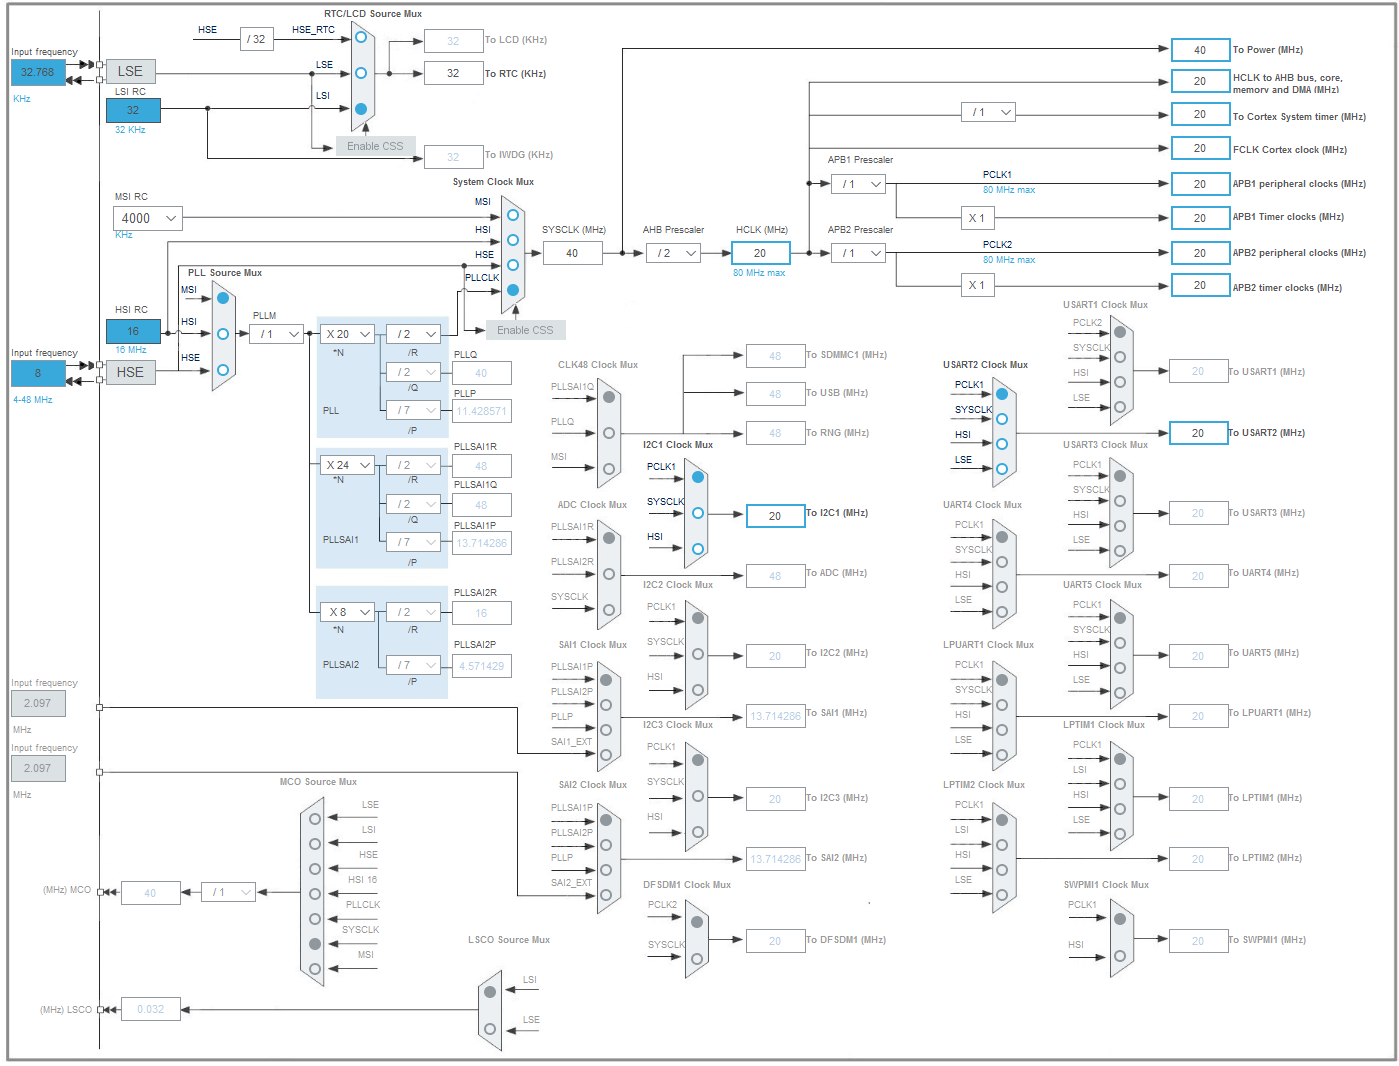
\includegraphics[width=0.9\textheight,angle=90]{konfiguracja_clk.png}
	\caption{Konfiguracja zegarów mikrokontrolera}
	\label{fig:KonfiguracjaZegara}
\end{figure}

%Obecne we wszystkich dokumentach
\subsection{Konfiguracja pinów}

\begin{table}[H]
	\centering
	\begin{tabular}{|l|l|l|l|}
		\hline
		Numer pinu	&	PIN & Tryb pracy & Funkcja/etykieta\\
		\hline
		8&	PC14 & OSC32\_IN &	RCC\_OSC32\_IN	\\
		9&	PC15 & OSC32\_OUT &	RCC\_OSC32\_OUT	\\
		12&	PH0 & OSC\_IN &	RCC\_OSC\_IN	\\
		13&	PH1 & OSC\_OUT &	RCC\_OSC\_OUT	\\
		39&	PE8 &	GPIO\_Output&	LD\_G [LED\_Green] \\
		47&	PB10 &	I2C2\_SCL&	\\
		48&	PB11 &	I2C2\_SDA&	\\
		86&	PD5 &	USART2\_TX&	USART\_TX\\
		87&	PD6 &	USART2\_RX&	USART\_RX\\
		92&	PB6 &	I2C1\_SCL&	\\
		93&	PB7 &	I2C1\_SDA&	\\
		\hline
	\end{tabular}
	\caption{Konfiguracja pinów mikrokontrolera}
	\label{tab:KonfiguracjaPinów}	
\end{table}

%Obecne we wszystkich dokumentach
\subsection{I2C}
\begin{table}[H]
	\centering
	\begin{tabular}{|l|c|} \hline
		\textbf{Parametr} & Wartość \\
		\hline
		\hline  \textbf{I2C Speed Mode}&Standard Mode  \\\hline
		\textbf{I2C Speed Frequency} & 100kHz\\
		\hline
	\end{tabular}
	\caption{Konfiguracja peryferium I2C}
	\label{tab:I2C}
\end{table}

\subsection{UART}
Peryferium skonfigurowano na potrzeby debugowania.
\begin{table}[H]
	\centering
	\begin{tabular}{|l|c|} \hline
		\textbf{Parametr} & Wartość \\
		\hline
		\hline  \textbf{Baud Rate}&\textcolor{blue}{9600}\\\hline
		\textbf{Word Length } & 8 Bits (including parity)\\\hline
		\textbf{Parity} &  None\\
		\hline
		\textbf{Stop Bits}& 1\\
		\hline
		\textbf{Data Direction}& Receive and Transmit\\
		\hline
	\end{tabular}
	\caption{Konfiguracja peryferium USART}
	\label{tab:USART}
\end{table}

\subsection{DMA}
\begin{table}[H]
	\centering
	\begin{tabular}{|l|c|} \hline
		\textbf{Parametr} & Wartość \\
		\hline
		\hline  \textbf{DMA request}& DAC\_CH1\\\hline
		\textbf{Stream} & DMA1\_Channel3\\
		\hline
		\textbf{Direction} & Memory To Peripheral\\
		\hline
	\end{tabular}
	\caption{Konfiguracja peryferium DMA}
	\label{tab:DAC}
\end{table}

%Obecne w dokumencie do etapu I
\section{Harmonogram pracy}

\begin{figure}[H]
	\centering
	\includegraphics[width=0.9\textwidth]{gantt_diagram.png}
	\caption{Diagram Gantta}
	\label{fig:DiagramGantta}
\end{figure}

Kolejne kamienie milowe pokrywają się z etapami wyszczególnionymi w podrozdziale Podział pracy.
%Obecne w dokumencie do etapu I
\subsection{Podział pracy}

\begin{table}[H]
	\centering
	\begin{tabular}{|L{7cm}|L{0.8cm}||L{7cm}|L{0.8cm}|}
		\hline
		\hline
		\textbf{Tomasz Masłoń} & 
		\% & 
		\textbf{Cyprian Hryniuk} & \%\\
		\hline
		\hline
		Wstępna konfiguracja peryferiów w programie CubeMx		& &	
		 	Wstępna konfiguracja peryferiów w programie CubeMx	&\\
		\hline
		Implementacja obsługi Audio DAC & &
		 	Implementacja obsługi czujników odległości&\\
		\hline
		Opracowanie algorytmu generujacego falę dźwiękową na podstawie danych z czujników odległosci & &
		Opracowanie algorytmu generującego falę dźwiękową na podstawie danych z czujników odległosci & \\
		\hline
		\end{tabular}
	\caption{Podział pracy -- Etap II}
	\label{tab:PodzialPracyEtap2}
\end{table}

\begin{table}[H]
	\centering
	\begin{tabular}{|L{7cm}|L{0.8cm}||L{7cm}|L{0.8cm}|}
		\hline
		\hline
		\textbf{Tomasz Masłoń} & 
		\% & 
		\textbf{Cyprian Hryniuk} & \%\\
		\hline
		\hline
		Finalna konfiguracja peryferiów w programie CubeMX		& &	
		Finalna konfiguracja peryferiów w programie CubeMX &\\
		\hline
		Opracowanie funkcji modyfikujacej brzmienie  & &
		Opracowanie funkcji modyfikującej brzmienie &\\
		\hline	
	\end{tabular}
	\caption{Podział pracy -- Etap III}
	\label{tab:PodzialPracyEtap3}
\end{table}


%Obecne we wszystkich dokumentach
\section{Podsumowanie}
Projekt dotyczy stworzenia instrumentu muzycznego - theremina, przy wykorzystaniu cyfrowych czujników odległościowych oraz AudioDAC

\newpage
\addcontentsline{toc}{section}{Bibilografia}
\bibliography{bibliografia}
\bibliographystyle{plabbrv}


\end{document}
